\documentclass[hidelinks,12pt,a4paper]{report}
\usepackage[utf8]{inputenc}
\usepackage{fontspec}
\usepackage{amsmath}
\usepackage{amsfonts}
\usepackage{amssymb}
\usepackage[margin=1in,left=1.2in,includefoot]{geometry}
% Algorithm
\usepackage{algorithm}
\usepackage{amssymb}
% IF else
\usepackage{algorithmic}
\usepackage[export]{adjustbox}
\usepackage{caption}
\usepackage{booktabs}
\usepackage{tabularx}
\newcolumntype{Y}{>{\raggedright\arraybackslash}X}
\usepackage{listings}
\usepackage{color}
\usepackage{makecell}

\definecolor{dkgreen}{rgb}{0,0.6,0}
\definecolor{gray}{rgb}{0.5,0.5,0.5}
\definecolor{mauve}{rgb}{0.58,0,0.82}

% color python code
\lstset{frame=tb,
  language=Python,
  aboveskip=3mm,
  belowskip=3mm,
  showstringspaces=false,
  columns=flexible,
  basicstyle={\small\ttfamily},
  numbers=none,
  numberstyle=\tiny\color{gray},
  keywordstyle=\color{blue},
  commentstyle=\color{dkgreen},
  stringstyle=\color{mauve},
  breaklines=true,
  breakatwhitespace=true,
  tabsize=3
}

% Hyperlinks
\usepackage[unicode]{hyperref}
% Graphic
\usepackage{graphicx}
\usepackage{subfig}
\usepackage{float}

%----------------------------------------------------------------------------------------
%	DOCUMENT INFORMATION
%----------------------------------------------------------------------------------------

\title{}
\author{Tu \textsc{Vu}}
\date{\today}

\begin{document}

\begin{titlepage}

\includegraphics[height=1.75cm, valign=c]{images/bordeaux_logo.jpg}
\hspace*{0.3cm}
\includegraphics[height=1.75cm, valign=c]{images/LaBRI_logo.jpg}
\hspace*{1.3cm}
\includegraphics[height=1.95cm, valign=c]{images/puf_logo.jpg}\\[1.5cm]
		
	\begin{center}
	
	%\textsc{\LARGE }\\[1.5cm] % Main heading such as the name of your university/college
	
	\textsc{\Large UNIVERSITY OF BORDEAUX}\\[1.5cm] % Major heading such as course name
	
	\textsc{\large INTERNSHIP REPORT}\\[1.5cm] % Minor heading such as course title


%{\large Final report}\\[0.5cm]	
	
	\line(1,0){400}\\[0.2in]
	\huge{\bfseries Deep Learning \\ Heritage Image Classification}\\
	\line(1,0){400}\\[1.5cm]
	\noindent	
	\begin{minipage}{0.4\textwidth}
		\begin{flushleft} \large
    	\emph{Student:}\\
    	Manh Tu \textsc{Vu}
		\end{flushleft}
	\end{minipage}
	\begin{minipage}{0.4\textwidth}
  		\begin{flushright} \large
    		\emph{Supervisor:} \\
    		Marie \textsc{Beurton-Aimar}
    		Van Linh \textsc{Le}
  		\end{flushright}
	\end{minipage}
	
	\vfill

% Bottom of the page
{\large \today}
	\end{center}
\end{titlepage}

\chapter*{Acknowledgements}

First of all, I would like to express my deepest gratitude to my two supervisors, Mrs. Marie BEURTON-AIMAR and Mr. Van Linh LE for their agreements, guide, and support during the planning and developing of my internship.
\\
\\
I would like to thank Mr Fabien BALDACCI for his generous help and comment during my work. I would like to thank the staffs, students in LaBRI, who helped, supported with the technique and providing me a professional working environment.
\\
\\
I would also like to thank all the professors in the University of Bordeaux and the PUF-HCM, who imparted a lot of knowledge about learning and researching. Finally, I would like to thank my family and colleagues for their support and encouragement through my study.

\clearpage

\chapter*{Abstract}

Deep Learning is a subfield of machine learning concerned with algorithms inspired by the structure and function of the brain called artificial neural networks.
\\
\\
Image classification is a field that has many applications in life. It could be useful to categorize images, provide only images which the user are interesting, protect the children from unwanted contents such as violent or sexual. 
\\
\\
Although it already has a lot of algorithms to solve the Image classification problem. However, those (algorithms) are hard to implement and just specific to some domains. With the advent of deep learning, this problem become more easier and obtained a high performance result\cite{o.a.b.penattik.nogueiraj.a.dossantos2015}.
\\
\\
The goal of my internship at LaBRI is research \& implement the Deep learning in Image classification to classify images from Heritage repository\footnote{\href{https://heobs.org}{https://heobs.org}}. Try to do in different approach, compare them and finally, choose the one which give the best result.
% Table content
\tableofcontents
\listoffigures
\thispagestyle{empty}
\clearpage

\chapter*{Introduction}
Heritage Observatory project has for aim to identify cultural and historical heritages, constitute a specific database, provide a data archive free for all. This platform allows us to receive the breaking news about cultural or historical heritage sites located in regions of the world that we are interesting. In order to do that, the platform will collect a huge of images about the cultural and historical heritage. The problem appears when we want to categorize those images into a specific classes when the image have no label and we can't looking to each of those images and categorize it by hand. We need to find a way to let the computer do it for us.
The aim of my internship is to implement a deep-learning algorithm to classify those images.
\\
\\
Image classification is the task of assigning an input image one label from a fixed set of categories. There are lots of classifiers that exists, but nowadays, neural networks and deep learning currently provide the best solutions to many problems in image and speech recognition, and in natural language processing.
\\
\\
Deep learning, is a part of machine learning and it gives techniques for learning in neural networks. Neural networks are inspired by the human system of neurons that is able to learn from observations. It is feed by labeled data and learns automatically from that. The most adapted neural network for image recognition is the convolutional neural network (CNN). It's adapted to the recognition of 4 classes: being, heritage, scenery and other. That's why it has been implanted.
\\
\\
Deep learning has two major categories of image classification techniques include unsupervised and supervised classification. With unsupervised classification, all images are unlabeled and we using deep learning to learn to inherent structure from the image input data while with supervised classification, all images are labeled and we using deep learning to learn to predict the output from the image input data.
\\
In this project, we'll implement both of those categories of image classification techniques and then compare the result to see which one are better to solve our problem.
\chapter{Context}
\section{Pôle Universitaire Français}
The Pôle Universitaire Français (PUF) was created by the intergovernmental agreement of VietNam and France in October 2004. With ambition is building a linking program between the universities in VietNam and the advanced programs of universities in France. There are two PUF’s center in VietNam: Pôle Universitaire Français de l’Universite Nationalé du Vietnam - Ha Noi located in Ha Noi capital (PUF-Ha Noi) and Pôle Universitaire Français de l’Universite Nationalé du Vietnam - Ho Chi Minh Ville located in Ho Chi Minh city (PUF-HCM).
\subsection{PUF-HCM}
PUF-HCM\footnote{\url{http://pufhcm.edu.vn}} is a department of VietNam National Univeristy at Ho Chi Minh city. From the first year of operations, PUF-HCM launched the quality training programs from France in VietNam. With target, bring the programs which designed and evaluated by the international standards for Vietnamese student. PUF-HCM always strive in our training work. So far, PUF-HCM have five linking programs with the universities in France, and the programs are organized into the subjects: Commerce, Economic, Management and Informatics. In detail:

\begin{itemize}
	\item Bachelor and Master of Economics : linking program with University of Toulouse 1 Captiole
	\item Bachelor and Master of Informatics: linking program with University of Bordeaux and University of Paris 6.
\end{itemize}
The courses in PUF-HCM are provided in French, English and Vietnamese by both Vietnamese and French professors. The highlight of the programs are inspection and diploma was done by the French universities.
\section{Laboratoire Bordelais de Recherche en Informatique}
The Laboratoire Bordelais de Recherche en Informatique (LaBRI)\footnote{\url{http://www.labri.fr}} is a research unit associated with the CNRS (URM 5800), the University of Bordeaux and the Bordeaux INP. Since 2002, it has been the partner of Inria. It has significantly increased in staff numbers over recent years.
In March 2015, it had a total of 320 members including 113 teaching/research staff (University of Bordeaux and Bordeaux INP), 37 research staff (CNRS and Inria), 22 administrative and technical (University of Bordeaux, Bordeaux INP, CNRS and Inria) and more than 140 doctoral
students and post-docs. The LaBRI’s missions are: research (pure and applied), technology application and transfer and training.
Today the members of the laboratory are grouped in six teams, each one combining basic research, applied research and technology transfer:
\begin{itemize}
	\item Combinatorics and Algorithmic
	\item Image and Sound
	\item Formal Methods
	\item Models and Algorithms for Bio-informatics and Data Visualisation
	\item Programming, Networks and Systems
	\item Supports and Algorithms for High Performance Numerical Applications
\end{itemize}
Within these team, research activities are conducted in partnership with Inria. Besides that, LaBRI also collaborate with many other laboratories and companies on French, European and the international.
\newpage
\section{Heritage Observation project}
Heritage Observatory is the project has for aim to identify cultural and historical heritages, constitute a specific database, provide a data archive free for all. This platform allows us to receive the breaking news about cultural or historical heritage sites located in regions of the world that we are interesting. In order to do that, the platform will collect a huge of images about the cultural, historical heritage and then classify them into different categories. \\\\
The Heritage repository contain a huge set of images about vietnamese human, statue, ancient artifacts, building, landscape, etc. But all of them are completed unlabeled. So, the question is: ``How we can classify those images to the right classes and automatic classify the new image, which the machine has never seen to the right class''.\\\\
The first attempt is to categorize those images into four different classes including:

\begin{description}
\item[Heritage] \hfill \\ A place of cultural, historical, or natural significance for a group or society.
\item[Beings] \hfill \\ Any form of life, such as a plant or a living creature, whether human or other animal.
\item[Scenery] \hfill \\ Any form of landscapes which show little or no human activity and are created in the pursuit of a pure, unsullied depiction of nature, also known as scenery.
\item[Other] \hfill \\ Any other type of image that doesn't represent a photograph, such as painting, illustration, any object.	
\end{description}

\newpage
\begin{center}
\begin{figure}[!htb]
\subfloat[]{%
\begin{minipage}{\linewidth}
  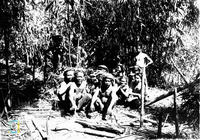
\includegraphics[width=5cm, height=3.5cm]{images/sample/being_6}\hfill
  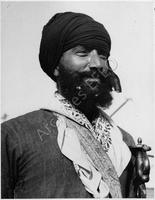
\includegraphics[height=3.5cm]{images/sample/being_35}\hfill
  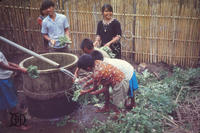
\includegraphics[width=5cm, height=3.5cm]{images/sample/being_45}%
\end{minipage}%
}\par
\subfloat[]{%
\begin{minipage}{\linewidth}
  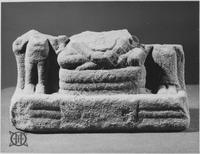
\includegraphics[width=5cm, height=3.5cm]{images/sample/heritage_145}\hfill
  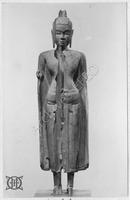
\includegraphics[height=3.5cm]{images/sample/heritage_147}\hfill
  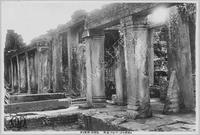
\includegraphics[width=5cm, height=3.5cm]{images/sample/heritage_282}%
\end{minipage}%
}\par
\subfloat[]{%
\begin{minipage}{\linewidth}
  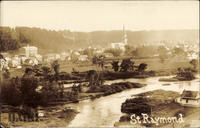
\includegraphics[height=2.8cm]{images/sample/scenery_111}\hfill
  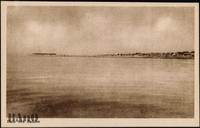
\includegraphics[height=2.8cm]{images/sample/scenery_102}\hfill
  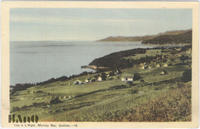
\includegraphics[height=2.8cm]{images/sample/scenery_110}%
\end{minipage}%
}\par
\subfloat[]{%
\begin{minipage}{\linewidth}
  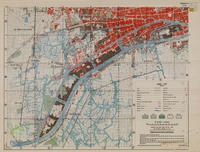
\includegraphics[width=5cm, height=3.5cm]{images/sample/other_129}\hfill
  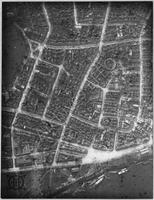
\includegraphics[height=3.5cm]{images/sample/other_190}\hfill
  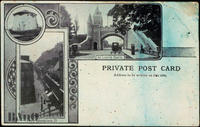
\includegraphics[width=5cm, height=3.5cm]{images/sample/other_202}%
\end{minipage}%
}
  \caption{Images from Heritage repository}
\end{figure}
\end{center}

\newpage
\section{The internship project}

The internship is intended to be a duration to apply academic knowledge to professional environment. It shows the ability synthesis, evaluation and self-research of student. Besides, the student may study the experience from the real working environment. My internship is done under the guidance of Mrs Marie BEURTON-AIMAR in a period of six months at LaBRI laboratory.\\\\
The objective of this internship is implementing a method to automatize the classification of images.\\\\
The goal is to use deep convolutional neural networks (CNNs or ConvNets) to tackle the remote sensing scene classification task.\\\\
\newpage

\chapter{Analysis}
\section{State of the art}
Labeling an image according to a set of semantic categories is the goal of image classification. This is a very challenging problem because of the characteristic of a given class may present a large variability and the objects may appear at different position, scales, and orientations. Moreover, the same objects can be found in images belonging to different classes.
\section{Scikit-learn algorithm cheat-sheet\cite{scikitlearn.org}}
Because it has many algorithms has able to classify images such as: Decision tree\cite{j.r.quinlan1985}, SVM\cite{stever.gunn1998}, K-nearest neighbors\cite{orenanavakfiry.levy2017}, etc. We need to find a right one to solve our problem. The Scikit-learn had made an algorithm cheat-sheet to help us to choose the right one:

\begin{figure}[ht]
	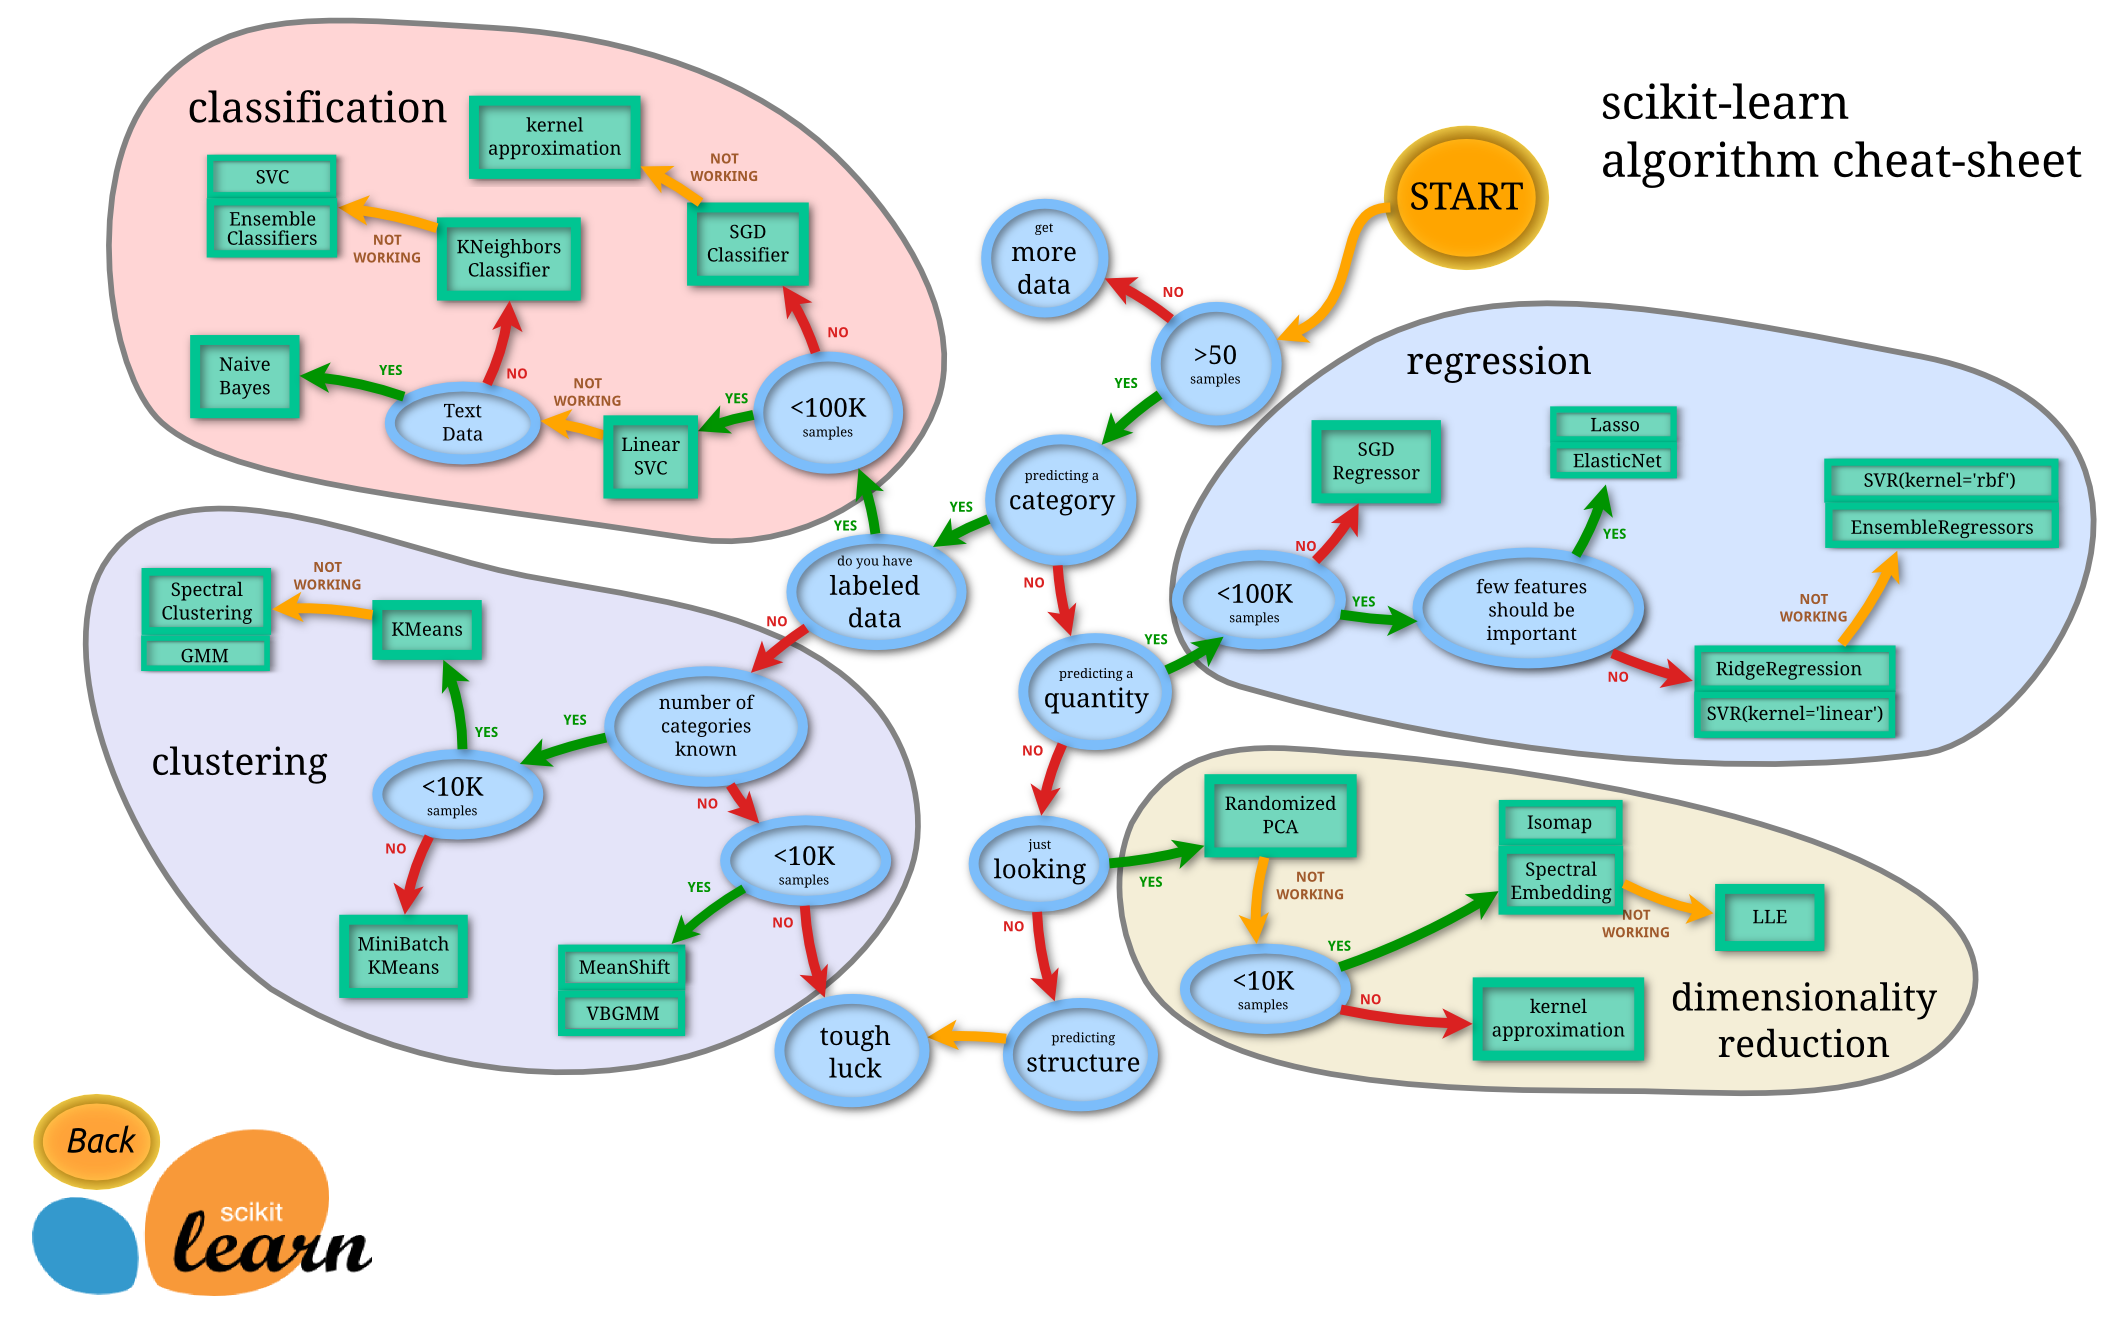
\includegraphics[width=\textwidth, center]{images/scikit-learn}
	\caption{Scikit-learn algorithm cheat-sheet}
	\label{fig:Scikit-learn}
\end{figure}
This algorithm cheat-sheet(see Fig \ref{fig:Scikit-learn}) suggests to use K-mean algorithm to classify our images because of unlabeled images and, the size of our dataset is less than 10K samples. However, one can note that it is mandatory to create a labeled dataset from our unlabeled images by hand and then, we can use SGD Classifier to do it.
\\
Finally, two ways are proposed to reach our goal: one is use Supervised Classification with SGD is our main algorithm. The other is use Unsupervised Classification with K-mean is main algorithm. Both of them can be applied by using Convolution Neural Network(CNN).
\section{General CNN architecture}
A convolutional network is a neural network that use convolutions. It is a multiplayer network (e. g. it uses several layers). In reality, those kind of network, are dividing in two part. The first one use convolutional layers - layers that use convolution patches to compute weights used in neurons. The second part, used to connect the first part to the output, is made of fully connected layers: every output of a layer is connected to every neurons of the next one without any distinctions.

\begin{figure}[ht]
	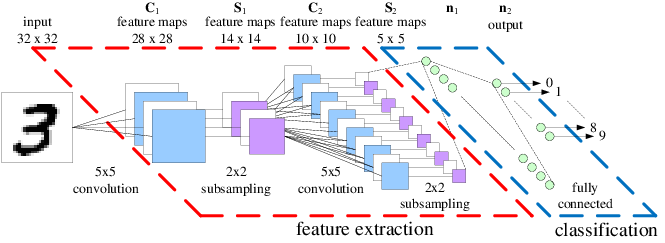
\includegraphics[scale=1, center]{images/Fig-1-An-Example-CNN-architecture-for-a-handwritten-digit-recognition-task}
	\caption{An Example CNN architecture for a handwritten digit recognition task.}
	\label{fig:CNN-architecture}
\end{figure}
The network architecture of an example CNN is depicted in Fig \ref{fig:CNN-architecture}. The processing starts with feature extraction layers and is finished by fully connected classification layers. Using different layers delivers robust recognition accuracy and is invariant to small geometric transformations of the input images. The robust recognition accuracy makes that CNN are successfully used for classification tasks on real world data
\newpage
\section{Libraries}
The fact is, we're unable to do eveything from scratch, CNN's too complex if we want to build it by our self. There have a several libraries for CNN, which developed by some researching labs, universities or companies to help us to make easy to construct and configure our model. Below is some of those libraries:
\begin{itemize}
	\item \textbf{Caffe}\footnote{\url{http://caffe.berkeleyvision.org}} a deep learning framework made with expression, speed, and modularity in mind.
	\item \textbf{Tensorflow}\footnote{\url{https://www.tensorflow.org}} an open source software library for numerical computation using data flow graphs.
	\item \textbf{Theano}\footnote{\url{http://deeplearning.net/software/theano}} CPU/GPU symbolic expression compiler in python (from MILA lab at University of Montreal)
	\item \textbf{Keras}\footnote{\url{https://keras.io}} a high-level neural networks API, written in Python and capable of running on top of TensorFlow, CNTK, or Theano.
	\item \textbf{Torch}\footnote{\url{http://torch.ch}} a scientific computing framework with wide support for machine learning algorithms that puts GPUs first. 
\end{itemize}

And much more other libraries. So, It’ll be hard to know that which one is the best. However, we all know that they will do well their job. The thing most important here is the network model and the configure parameters. \\
\\
So, after some researched, we found many papers, articles relevance with our problem such as: \cite{placesdatabase}, \cite{landclassification}. They implemented Caffe Library. So, we choose \textbf{Caffe} as our library to represent the CNN model since it’s one of the most popular libraries for deep learning (convolutional neural networks in particular). It's developed by the Berkeley Vision and Learning Center (BVLC) and
community contributors. It’s easily customizable through configuration files, easily extendible with new layer types,
and provides a very fast ConvNet implementation (leveraging GPUs, if present). It provides C++, Python and MATLAB APIs.

\newpage

\section{The ImageNet Visual Recognition Challenge}

The ImageNet Visual Recognition Challenge\footnote{\url{http://www.image-net.org/challenges/LSVRC/2012}} is a competition where research teams evaluate their algorithms on the given data set, and compete to achieve higher accuracy on several visual recognition tasks such as Classification, Classification with localization or Fine-grained classification. \\
Because they have the same kind of goal with our project, so, we will try to implement the CNN model of the winner of this challenge and also try to improve it to get the better result.

\chapter{Conception}

\chapter{Realization}
\section{The Dataset}
\label{chap:dataset}
Because both Supervised and Unsupervised Classification are required a dataset to train and test, this chapter describes how we obtain and optimize the dataset.
\subsection{Fetch all images}
The entire image dataset described on the text file named ”photos.txt” line by line. Each line includes the image id and image description as below:
\begin{verbatim}
5a36f382-dbdf-11e6-95fd-d746d863c3eb | Những người ăn xin  | vie
5a36f382-dbdf-11e6-95fd-d746d863c3eb | Mendiants  | fra
17be8122-dbe0-11e6-860c-5fea02802d0a | Chợ Cũ (3) | vie
17be8122-dbe0-11e6-860c-5fea02802d0a | Vieux marché (3) | fra
400286c8-dbe1-11e6-bb4d-ff975c68de04 | Ngân hàng Đông Dương  | vie
400286c8-dbe1-11e6-bb4d-ff975c68de04 | La Banque de l’Indochine  | fra
\end{verbatim}
In order to get the image dataset, we have to fetch each image one by one by join the image id with heobs cdn url \href{https://cdn.heobs.org/photo/}{https://cdn.heobs.org/photo/}. For example, with the first line in the record above, we have the following URL: 
\begin{verbatim}
https://cdn.heobs.org/photo/5a36f382-dbdf-11e6-95fd-d746d863c3eb
\end{verbatim}
We wrote a python script to automatic read this text file \& download images one by one.
Totally, we have 142459 images in our dataset.

\subsection{Remove broken images}
After downloaded \& look around all images, we found that it has a lot of broken images, which can't be displayable. So, we write a python script to filter all of those broken images automatically. \newline
Finally, we have 89850 images left in our dataset.

\subsection{Labeling image dataset}
It's mandatory to label our images for both Supervised and Unsupervised Classification because with Unsupervised Classification, we need a labeled dataset to validate if the image is classified correct or not. With Supervised Classification, we need a labeled dataset to train \& validate the Neural Network Model.\newline\newline
Before labeling our images by hand, we need to build a good images dataset, which has the same image resolution. We loop through all our images to filter all images, which has the most common image resolution and reject all others. After this step, we have 55143 images left. \newline\newline
Finally, we labeling our images by hand and completed our dataset as the table below:\newline\newline
{\renewcommand{\arraystretch}{2}%
\noindent\begin{tabularx}{\textwidth}{YYYY}
  \hline
& Being & Heritage & Scenery\\
N\textsuperscript{o} images & 1471 & 1832 & 942\\
 \hline
\end{tabularx}} \quad

\section{Unsuppervised Deep Learning}

Because of when classifying images by hand, it has some special case when one image may refer to more than one class. Thus, we need the machine to help us to make decisions by comparing two images are the same class or not. We also want to separate images of one class into multi unknown sub-classes. So, by using Unsupervised Deep Learning, we want to let the machine to classify a set of images unlabeled into some unknown classes. \newline\newline
After some researches about this problem, we found the Unsupervised Deep Embedding for Clustering Analysis (DEC)\cite{dec} paper, which propose a new method that simultaneously learns feature representations and cluster assignments using deep neural networks to classify unlabeled images.\newline\newline
The DEC has two phases:
\begin{description}
\item[Phase 1:]  Parameter initialization with a deep autoencoder
\item[Phase 2:]  Parameter optimization (i.e., clustering)
\end{description}
We already tried to run this implement code with the latest Caffe version (Jul 2017), but it doesn't work because this Caffe model required some deprecated model parameters. However, because of the code delivery with Caffe and Docker, so, we continue to try with Docker and their 
Caffe version.\newline\newline
The Dockerfile in the original source code has exception but fixed by the following patch:
\begin{verbatim}
 -  liblmdb-dev libboost1.54-all-dev libatlas-base-de
 +  liblmdb-dev libboost1.54-all-dev libatlas-base-dev
\end{verbatim}
\subsection{Trying to run DEC with MNIST dataset}
We'll first try to test with MNIST dataset - the simplest example provided with the source code.\newline
In parameter optimization phase, they use KMeans Cluster to try to predict the closest cluster each sample in the test image belongs to. The most important part of this phase is:
\begin{lstlisting}
if (Y_pred != Y_pred_last).sum() < 0.001*N:
    print acc_list
    return acc, nmi
\end{lstlisting}
This is the terminate, the application achive the goal when the current predict (Y\_pred) is not different with the last predict. The value 0.001*N is threshold.
\subsubsection{Generate the test summary result}
Currently, the code just show the accuracy of the whole process. We need to write we own function to calculate the accuracy of each classes.
Because with mnist dataset, we already have the correct label of each image. So, to be able to summary the result, we add the following function to compare between predict \& actual result:

\begin{lstlisting}
def show_result(predicts, actuals):
    summary = {}
    for idx, value in enumerate(actuals):
        actual = str(value)
        predict = str(predicts[idx])
        if actual in summary:
            if predict in summary[actual]:
                summary[actual][predict] += 1
            else:
                summary[actual][predict] = 1
        else:
            summary[actual] = {}
    print summary
\end{lstlisting}
And call this function when the application predict done
\begin{lstlisting}
if (Y_pred != Y_pred_last).sum() < 0.001*N:
     classify_dataset(Y_pred, img, db)
     show_result(Y_pred, Y)
     print acc_list
     return acc, nmi
\end{lstlisting}

\subsubsection{Classify image dataset into X classes}
This feature put the images from dataset, which has the same class into one folder. This helps us to easy to verify the classification result

\begin{lstlisting}
def classify_dataset(predicts, imgs, db):
    classes_dir = "classes_" + db
    if not os.path.isdir(classes_dir):
        os.makedirs(classes_dir)
    for idex, pred in enumerate(predicts):
        tmp_dir = os.path.join(classes_dir, str(pred))
        if not os.path.isdir(tmp_dir):
            os.makedirs(tmp_dir)
        dispSingleImg(imgs, idex, os.path.join(tmp_dir, str(idex) + ".jpg"))
\end{lstlisting}
We call this function when the application predict done
\begin{lstlisting}
if (Y_pred != Y_pred_last).sum() < 0.001*N:
     classify_dataset(Y_pred, img, db)
     print acc_list
     return acc, nmi
\end{lstlisting}

\subsubsection{Convert binary images into displayable images}
Because of the images used in the application is stored in binary \& read directly into memory. So, to be able to get the classified result, we've to convert image stored in memory (RAM) to the displayable image file. 

\begin{lstlisting}
def dispSingleImg(X, n, fname=None):
    h = X.shape[1]
    w = X.shape[2]
    c = X.shape[3]
    buff = np.zeros((h, w, c), dtype=np.uint8)

    buff[0:h, 0:w, :] = X[n]

    if fname is None:
        cv2.imshow('a', buff)
        cv2.waitKey(0)
    else:
        cv2.imwrite(fname, buff)
\end{lstlisting}
\begin{description}
\item[X:] array of image dataset
\item[n:] index of image
\item[fname:] destination to save
\end{description}

\subsubsection{Acquire and analytics the test result}
After run this network model with the \textbf{init.caffemodel}, we acquire the result describe as the following table:
\begin{table}[H]
\begin{center}
\begin{tabular}{| c | c | c | c | c | c | c | c | c | c | c |}
\hline
 & Predict 0 & 1 & 2 & 3 & 4 & 5 & 6 & 7 & 8 & 9\\
\hline
Actual 0 & 17 & 35 & 53 & 15 & 1 & 141 & 6629 & 1 & 4 & 6\\
\hline
1 & 7658 & 14 & 16 & 8 & 153 & 3 & 1 & 9 & 2 & 3\\
\hline
2 & 278 & 15 & 20 & 229 & 6094 & 42 & 73 & 29 & 112 & 87\\
\hline
3 & 108 & 128 & 13 & 178 & 171 & 6 & 12 & 23 & 67 & 6434\\
\hline
4 & 65 & 8 & 3060 & 8 & 7 & 58 & 3 & 3612 & 4 & 0\\
\hline
5 & 60 & 4968 & 41 & 133 & 6 & 54 & 7 & 37 & 13 & 899\\
\hline
6 & 233 & 268 & 2 & 37 & 14 & 6124 & 187 & 9 & 0 & 1\\
\hline
7 & 251 & 16 & 336 & 17 & 103 & 1 & 22 & 317 & 6226 & 3\\
\hline
8 & 167 & 142 & 62 & 5922 & 32 & 36 & 73 & 72 & 23 & 295\\
\hline
9 & 80 & 12 & 3624 & 60 & 5 & 16 & 47 & 2910 & 97 & 106\\

\hline
\end{tabular}
\caption {Mnist init.caffemodel test result}
\end{center}
\end{table}

Because Unsupervised Classification don't know what classes actually are. It just grouping the images, which it think there's the same into one class. So, we've to figure what these classes are.

\begin{figure}[H]
\centering
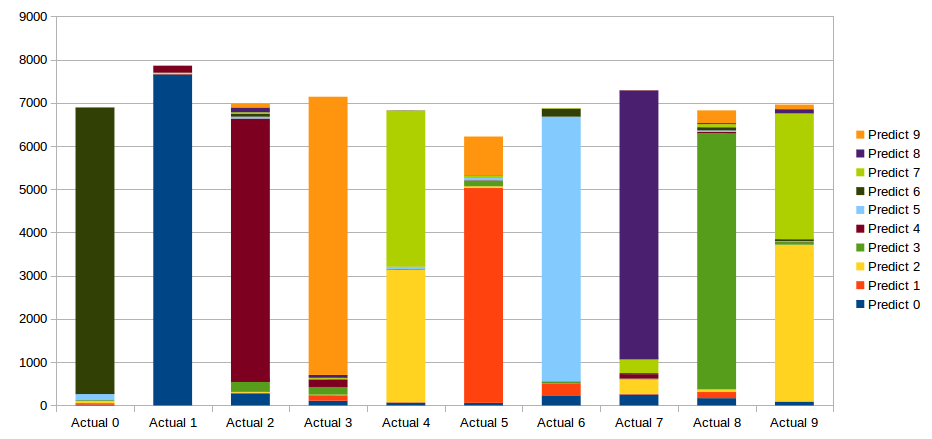
\includegraphics[width=1\textwidth]{images/mnist_test_result_2}
\caption{Mnist init.caffemodel test result - correct}
\label{fig:samplepagoda}
\end{figure}

As the result above, we can easy to figure out that almost it can predict the images belong to which classes in high performance. Although it has a little confuse when predicting 2 and 7 but we can understand because of this two digit is similar.

Now we know how to receive the result of this implement source code. However, because of Mnist dataset is too simple. It just contains images, which has 28x28 pixel and only black \& white colors while our image Dataset has both bigger and true color. So, we need to try with the more complex Dataset. 

\subsection{Trying to run DEC with STL dataset}
In the test datasets they provide us has STL dataset, which closest with our Dataset (96 x 96 pixel, true color). We're going to try with this Dataset before try with we own dataset.\\\\
The application failure when execute \textbf{make\_stl\_data.py} python file to create STL LevelDB because of the "features.pyx" file is not delivery with the source code. 
The author of DEC mention to this file located at pyvision project\footnote{\href{https://github.com/cvondrick/pyvision/blob/master/vision/features.pyx}{https://github.com/cvondrick/pyvision/blob/master/vision/features.pyx}}. However, when testing this file, we got another error message:
\begin{verbatim}
Type Error: "int" object is not iterable
\end{verbatim}
As the author say "It's been too long and I almost forgot about it, sorry. But you can try to refer to stackoverflow. I believe you can find your answer"\footnote{\href{https://github.com/piiswrong/dec/issues/1}{https://github.com/piiswrong/dec/issues/1}}. So, after some debug \& research, we found that the problem caused by the parameter of \textbf{function hog} in \textbf{feature.pyx} is an image object. But we provided an numpy object. So, we fixed it by replaced the following line in \textbf{features.pyx}
\begin{verbatim}
line 48. 		with, height = im.size
\end{verbatim}
by the following line:
\begin{verbatim}
line 48. 		with, height = im.shape[:2]
\end{verbatim}
Finally, it works. The accuracy result is 35.7\% (35.9\% in the paper).

\subsection{Preparing we own image dataset}
Because the program require our dataset must be on LevelDB database and in specific format. However, our dataset just contain raw images. So, we have to write we own function to convert our dataset to ther dataset format.\newline\\
Below is the code we using to generate \& save data into LevelDB:
\begin{lstlisting}
import sys
import os
import Image
import numpy as np
import cv2
import cv
from joblib import Parallel, delayed
import features
import random
import dec
import pdb

def mode():
    if "MODE" in os.environ:
        return os.environ['MODE']
    return 'validate'


def load_data(images_dir):
    ims = [read(os.path.join(images_dir, filename)) for filename in os.listdir(images_dir)]
    X = np.array(ims, dtype='uint8')
    n_jobs = 10
    cmap_size = (6, 10)
    N = X.shape[0]

    H = np.asarray(Parallel(n_jobs=n_jobs)(delayed(features.hog)(X[i]) for i in xrange(N)))

    H = H.reshape((H.shape[0], H.size / N))

    X_small = np.asarray(Parallel(n_jobs=n_jobs)(delayed(cv2.resize)(X[i], cmap_size) for i in xrange(N)))
    crcb = np.asarray(Parallel(n_jobs=n_jobs)(delayed(cv2.cvtColor)(X_small[i], cv.CV_RGB2YCrCb) for i in xrange(N)))
    crcb = crcb[:, :, :, 1:]
    crcb = crcb.reshape((crcb.shape[0], crcb.size / N))

    feature = np.concatenate(((H - 0.2) * 10.0, (crcb - 128.0) / 10.0), axis=1)
    print feature.shape

    return feature, X[:, :, :, [2, 1, 0]]


def load_label(images_dir, classes, determine):
    return np.array([get_label(classes, filename, determine) for filename in os.listdir(images_dir)], dtype='uint8')


def get_label(classes, filename, determine):
    if mode() == 'validate':
        return classes.index(filename.split(determine)[0])
    return 0


def load_named_label(images_dir):
    return np.array([filename for filename in os.listdir(images_dir)], dtype='str')

if __name__ == '__main__':
    classes = ["heritage", "being", "scenery"]
    images_dir = sys.argv[1]
    read = lambda imname: np.asarray(Image.open(imname).convert("RGB"))
    if os.path.isdir(images_dir):
        X_train, img_train = load_data(images_dir)
        Y = load_label(images_dir, classes, "_")
        labeled = load_named_label(images_dir)
        p = np.random.permutation(X_train.shape[0])
        X_total = X_train[p]
        Y_total = Y[p]
        labeled_total = labeled[p]
        np.save("custom_named_label", labeled_total)
        img_total = img_train[p]
        dec.write_db(X_total, Y_total, 'custom_total')
        dec.write_db(img_total, Y_total, 'custom_img')
        N = X_total.shape[0] * 4 / 5
        dec.write_db(X_total[:N], Y_total[:N], 'custom_train')
        dec.write_db(X_total[N:], Y_total[N:], 'custom_test')
    else:
        raise Exception("Please specific image url")


\end{lstlisting}
The dataset must contain all images in the same root folder and each images in the dataset must have the following format :
\begin{verbatim}
<image class>_<index>.jpg
\end{verbatim}
Run the following command in the source root to create our custom dataset: 
\begin{verbatim}
python make_data.py <image dataset path>
\end{verbatim}
\subsection{Train with our dataset}
After train with our dataset, we get accurency 68.74\%

\begin{figure}[H]
\centering
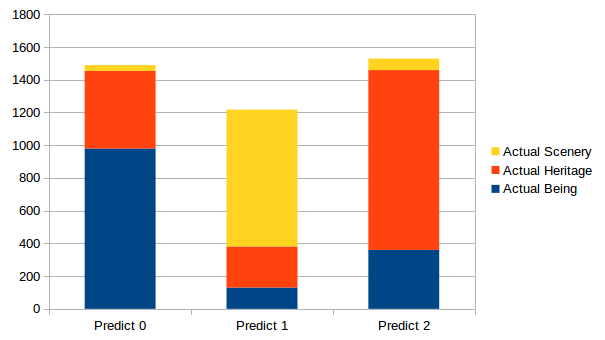
\includegraphics[width=1\textwidth]{images/unsupervised_large_dataset_result}
\caption{Unsupervised train result}
\end{figure}

\subsection{Classify the whole images}
..........................
\section{Suppervised Deep Learning}
Supervised deep learning requires us to provide a training dataset, which includes a list of images labeled. However, our images are not, and we can't classify the entire dataset by hand. So, we propose the following method, which includes three steps:
\begin{itemize}
\item Train a Convolution Neural Network (CNN) model with a part of images based on the original images, which we already done in \autoref{chap:dataset}
\item Use the CNN model trained above to classify the entire original images
\item Calculate the performance of the classification by random images in each class to review
\end{itemize}

\bibliographystyle{ieeetr}
\bibliography{bibfile}
\end{document}